\chapter{User Interface}

The user interface consists of a top bar, a status bar in the bottom,
the Scene Viewport and the Node Graph Editor with the Graph Menu Bar.
When the software is loaded the Node Graph Editor is shown. On the top left
of the graph editor there is an arrow that can be used to minimize it,
revealing the Scene Viewport behind it. The top bar and the status bar are
always visible.

\section{Node Graph Editor}
\begin{figure}[H]
\centering
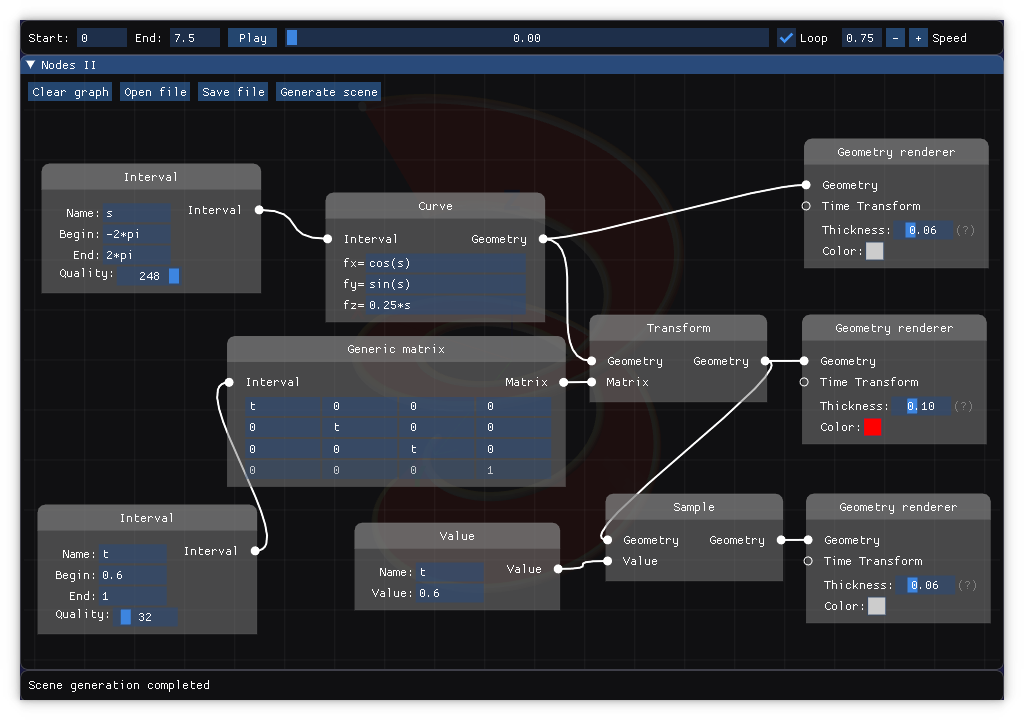
\includegraphics[width=0.666\textwidth]{figures/graph_editor.png}
%\caption{\label{fig:topbar}}
\end{figure}
The Node Graph Editor is where most of the work is done.
Each node represents an operation that creates or modifies data. Besides the inputs and
the output, many nodes also have internal fields in which the user can write an expression
or choose a value for a given property (e.g. a function, or ``$pi/4$'' for an angle).

The user can perform the following:
\begin{itemize}
    \item To add a node, simply right-click on empty space inside the node graph editor;
            a popup menu will open to display all the available node types, grouped by categories.
            See the following section for a detailed explaination of all menu entries.

    \item To move a node around, left click on its header and drag it to its new position.

    \item You can select a group of nodes by left-clicking on empty space and dragging the mouse,
            or by clicking on nodes while holding the \texttt{ctrl} key, to move all of them together.

    \item To remove a node, right-click on its header and select ``delete'' from the dropdown menu.

    \item To connect two nodes, hover over an input or an output. When the label turns blue, click it
            and drag with the mouse to the label of the output or input that you want to connect to. 

    \item To remove a connection, double-click it or hover and press the \texttt{delete} key

    \item The user can pan around the graph by right-clicking on empty space and dragging with the mouse,
            or by using the mouse scroll/holding the \texttt{shift} key and using the mouse scroll.

    \item The user can zoom in or out my holding the \texttt{ctrl} key and using the mouse scroll.
        clicking the mouse scroll (a.k.a. \texttt{Mouse3} button) will reset the zoom level to 1.

\end{itemize}

\begin{figure}[H]
\centering
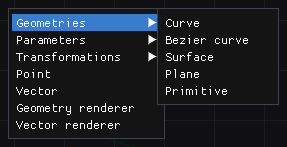
\includegraphics[width=0.4\textwidth]{figures/right_click_popup.png}
\caption{\label{fig:rightclick_manu} The right-click menu, with the ``Geometry'' submenu open}
\end{figure}

\subsection{Geometry submenu}
The geometry submenu contains the following nodes:

\subsubsection{Curve}

\hspace{\baselineskip}
\begin{tabular}{g|l}
    \hline
    Inputs: & Interval              \\
    \hline
    Fields: & fx, fy, fz            \\
    \hline
    Output: & a 1D Geometry object  \\
    \hline
\end{tabular}
\vspace{5pt}

This node is used to create a parametric curve using the input parameter Interval
and the given expressions for fx, fy and fz. Simple to use,
just make sure that the expressions are using the correct parameter name
(i.e. the same name used by the input Interval)

\subsubsection{Bezier}

\hspace{\baselineskip}
\begin{tabular}{g|l}
    \hline
    Inputs: & 2, 3 or 4 Points (0D Geometry objects)\\
    \hline
    Fields: & Quality\\
    \hline
    Output: & a 1D Geometry object\\
    \hline
\end{tabular}
\vspace{5pt}

This node uses its inputs as control points for a Bezi\`er curve. The degree of the
curve depends on how many inputs have been connected and empty inputs are ignored.
The Quality field determines the quality of the numerical approximation
of the ideal Bezi\`er curve.

\subsubsection{Surface}

\hspace{\baselineskip}
\begin{tabular}{g|l}
    \hline
    Inputs: & 2 Intervals\\
    \hline
    Fields: & fx, fy, fz\\
    \hline
    Output: & a 2D Geometry object\\
    \hline
\end{tabular}
\vspace{5pt}

Similarly to the curve one, this node can be used to create a parametric surface
given two Intervals and the given expressions for fx, fy and fz.
Both intervals are required and the user should use both of them:
if one parameter is never used in the expressions, it is likely that no visual output
will be produced, since a degenerated surface will be created.

\subsubsection{Plane}

\hspace{\baselineskip}
\begin{tabular}{g|l}
    \hline
    Inputs: & 1 point (0D Geometry), 1 Vector\\
    \hline
    Fields: & none\\
    \hline
    Output: & a Mesh Geometry object\\
    \hline
\end{tabular}
\vspace{5pt}

This node takes one point and a normal vector to create a special representation
of a plane. In particular, the representation consists of an evely-spaced grid centered
about the point given as input.

Please note the output is \textbf{not} a 2D Geometry, but a Mesh Geometry,
this means that you will not be allowed to apply a parametric transform
or a sample operation to a it, only a constant-valued transform can be applied.
This is because the purpose of this node is to have something useful for
visualization purposes, not to have a built-in parametric plane.

\subsubsection{Primitive}

\hspace{\baselineskip}
\begin{tabular}{g|l}
    \hline
    Inputs: & none\\
    \hline
    Fields: & Kind (a drop-down menu), Size\\
    \hline
    Output: & a Mesh Geometry object\\
    \hline
\end{tabular}
\vspace{5pt}

This node allows the user to create a basic primitive of the given kind
(Cube, Sphere, Cylinder, Cone, Pyramid or Dice). The Size fields allows
adjusting the primitive dimensions. See the question mark next to the 
slider for a description of how this value effects the output.

Just like the Plane node, the output is a Mesh Geometry, which is useful
for quick visualization or similar purposes. Parametric transforms
on these objects are not allowed.

\subsection{Parameters submenu}
This submenu contains all the nodes related to parameters

\subsubsection{Interval}

\hspace{\baselineskip}
\begin{tabular}{g|l}
    \hline
    Inputs: & none\\
    \hline
    Fields: & Name, Begin, End, Quality\\
    \hline
    Output: & Interval\\
    \hline
\end{tabular}
\vspace{5pt}

This node defines a parameter. By assigning a name, you will then be able
to use this parameter in expressions for parametric curves, surfaces and matrices.
Begin and End define the closed range in which the parameter lives, while Quality
allows the user to choose how many discretization points will be used when creating
a curve or a surface out of this parameter.

\subsubsection{Value}

\hspace{\baselineskip}
\begin{tabular}{g|l}
    \hline
    Inputs: & none\\
    \hline
    Fields: & Name, Value\\
    \hline
    Output: & Parameter Value\\
    \hline
\end{tabular}
\vspace{5pt}

In a similar way to the Interval node, the Value node lets you define a parameter
and assign a specific value to it. You can use it either as a ``variable''
to be used as input for a Matrix (e.g. define theta and then use it as a generic
angle inside the matrix expressions) or as an input to the Sample Parameter node.

\subsubsection{Sample Parameter}

\hspace{\baselineskip}
\begin{tabular}{g|l}
    \hline
    Inputs: & 1D or 2D Geometry object, Parameter Value\\
    \hline
    Fields: & none\\
    \hline
    Output: & 0D or 1D Geometry object\\
    \hline
\end{tabular}
\vspace{5pt}

The parameter sampling operation allows you to ``downgrade'' the dimension of a parametric
Geometric object, by assigning a parameter the value given as input.

In order for the operation to succeed, the Geometry must have a parameter with the same name
as to the one used in the Value input (e.g. if a surface is $S(p, q)$, the input value cannot
named $r$, only $p$ or $q$ will be accepted). The value must also be inside
the parameter's range. Please note that 1D Geometry created with the Bezi\`er
curve uses a hidden parameter name, and cannot therefore be sampled.

\subsection{Transformations submenu}
This submenu contains all nodes used to define transformation matrices and to
apply them to geometry objects.

\subsubsection{Generic Matrix}

\hspace{\baselineskip}
\begin{tabular}{g|l}
    \hline
    Inputs: & Parameter (either Interval or Value), optional\\
    \hline
    Fields: & matrix elements\\
    \hline
    Output: & Matrix object\\
    \hline
\end{tabular}
\vspace{5pt}

This node is used to define a generic Matrix, by writing one expression for each
matrix element. If an Interval is given as an input, then the output matrix will be
a parametric one.
Note that due to the nature of the software, there is no way to define a projection matrix,
since the last row of the matrix is fixed and cannot be modified.

As usual, if you provide a parameter as an input, make sure you
will be actually using it inside the expressions to prevent any kind of visualization
issue.

\subsubsection{Rotation Matrix}

\hspace{\baselineskip}
\begin{tabular}{g|l}
    \hline
    Inputs: & none\\
    \hline
    Fields: & Axis (drop down menu), Angle\\
    \hline
    Output: & Matrix object\\
    \hline
\end{tabular}
\vspace{5pt}

This node allows the user to quickly define a matrix which represents a rotation
of Angle radians around the chosen Axis.

\subsubsection{Translation Matrix}

\hspace{\baselineskip}
\begin{tabular}{g|l}
    \hline
    Inputs: & Vector\\
    \hline
    Fields: & none\\
    \hline
    Output: & Matrix Object\\
    \hline
\end{tabular}
\vspace{5pt}

Similarly to the previous, this node allows the user to quickly define a translation
matrix given the input Vector

\subsubsection{Transform}

\hspace{\baselineskip}
\begin{tabular}{g|l}
    \hline
    Inputs: & Geometry object, Matrix object\\
    \hline
    Fields: & none\\
    \hline
    Output: & Geometry object\\
    \hline
\end{tabular}
\vspace{5pt}

This node takes a matrix and applies it to a geometry, returning the transformed geometry.
If the input matrix was a parametric matrix, then a parametric transformation will be applied.
Please note that a parametric transform is not ``blindly'' applied to an object: if we have
a parametric curve or surface that depends on the same parameter used by the matrix,
the output geometry will still be a curve or a surface, modified accordingly
(e.g. applying a translation to a circle may output a spiral)

\subsubsection{Time Transform}

\hspace{\baselineskip}
\begin{tabular}{g|l}
    \hline
    Inputs: & none\\
    \hline
    Fields: & matrix elements\\
    \hline
    Output: & Time Transform object\\
    \hline
\end{tabular}
\vspace{5pt}

This node creates a Time Transform object, read th paragraph in the Data Types
section for more informations. All the expressions for the matrix elements
can contain the parameter $t$, i.e. ``time''.

\subsection{Point}

\hspace{\baselineskip}
\begin{tabular}{g|l}
    \hline
    Inputs: & none\\
    \hline
    Fields: & $x$, $y$, $z$\\
    \hline
    Output: & 0D Geometry object\\
    \hline
\end{tabular}
\vspace{5pt}

A very simple node to create a point. The implicit $w$ coordinate is set to $1$

\subsection{Vector}

\hspace{\baselineskip}
\begin{tabular}{g|l}
    \hline
    Inputs: & none\\
    \hline
    Fields: & $x$, $y$, $z$\\
    \hline
    Output: & Vector object\\
    \hline
\end{tabular}
\vspace{5pt}

A very simple node to create a Vector. As described in the data types section, a vector
is to be interpreted as a ``direction'', and the implicit $w$ coordinate is set to $0$

\subsection{Geometry Renderer}


\hspace{\baselineskip}
\begin{tabular}{g|l}
    \hline
    Inputs: & Geometry, Time Transform\\
    \hline
    Fields: & Thickness, Color\\
    \hline
    Output: & none\\
    \hline
\end{tabular}
\vspace{5pt}

This node is the one responsible for taking a Geometry object and rendering it to the screen.
Every frame the the Time Transform is applied to the it before rendering, by evaluating the
transform with a different value of $t$. The user can choose what color to use for any kind
of Geometry, while the Thickness value only effects the display of 1D geometries (curves).

\subsection{Vector Renderer}

\hspace{\baselineskip}
\begin{tabular}{g|l}
    \hline
    Inputs: & Point, Vector\\
    \hline
    Fields: & Thickness, Color\\
    \hline
    Output: & none\\
    \hline
\end{tabular}
\vspace{5pt}


This node is used to display a Vector, by representing it as an arrow.
Since a Vector is only a direction, the user must also provide the application point (i.e: the "tail") of the vector.
Just like with the Geometry Renderer, one can choose a color and the thickness of the arrow.

\section{Top Bar}

\begin{figure}[H]
\centering

\includegraphics[width=1.0\textwidth]{figures/top_bar.png}
%\caption{\label{fig:topbar} The right-click menu, with the ``Geometry'' submenu open}
\end{figure}

As it was explained before, any Geometry Renderer can have a Time Transform attached to it.
This time transform contains a parameter named $t$ that will changes in real time while the
user interacts with the rendered scene, as opposed to all other parameters that are evaluated
only once when the scene is generated.
The Top Bar gives the user control over the value of this parameter $t$.

\begin{itemize}
    \item Start: the expression for the beginning of the parameter interval. To use
        the constant $\pi$, write it as \texttt{pi}.
    \item End: the expression for the end of the parameter interval.
    \item Play/Pause: by clicking ``Play'' the parameter $t$ will increment at the given speed,
        while by clicking ``Pause'' the parameter will stay frozen to the value selected by the user.
    \item slider: the user can click and drag the slider to manually assign a value to $t$
    \item Loop checkbox: as the name implies, if this box is ticked the animation will loop
        (i.e. every time $t$ reaches the end of the interval, it will be rewinded to the start)
    \item Speed: the speed at which $t$ advances when ``Play'' is clicked. Defaults to $0.75$,
        meaning that 1 second of wall clock time will advance $t$ by $0.75$. The user can either
        write down the speed or click on the \texttt{+/-} signs to increase in small steps.
        Negative speeds are allowed!
\end{itemize}


\section{Graph Menu Bar}

\begin{figure}[H]
\centering
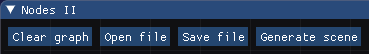
\includegraphics[width=0.5\textwidth]{figures/graph_menu_bar.png}
%\caption{\label{fig:topbar} The right-click menu, with the ``Geometry'' submenu open}
\end{figure}

The Graph Menu Bar contains 4 buttons, which function is easy to guess by their labels:

\begin{itemize}
    \item Clear Graph: deletes all nodes and connections.
    \item Open File: clears the graph and loads a previously saved file.
    \item Save File: saves the current graph to a file.
    \item Generate Scene: when the user is done modifying the graph, clicking this
        will trigger the generation of the scene.
\end{itemize}

Clearing the graph, opening or saving a file will open a dialog asking to confirm the operation.
In particular, when saving a file the extension \texttt{.toml} will be automatically added if
the name does not contain it, and if any name conflict arises, then the user will be asked if
the software should overwrite the file or cancel the operation.

\section{Scene Viewport}

After the scene is generated, the Graph Editor is minimized and the scene containing the generated
geometries is shown. Navigation is very easy, left-click and drag to rotate the view or use
the mouse scroll to zoom in and out. Currently it is not possible to pan around the scene.
The lights in the scene are placed in specific points to make sure that it is easier to understand
the shapes one is looking at. However, this also means that some combinations of shape and colors
might produce very dark spots in some geometries.

\section{Status Bar}

\begin{figure}[H]
\centering
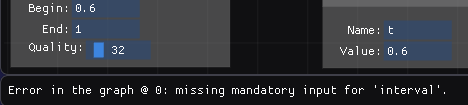
\includegraphics[width=0.6\textwidth]{figures/status_bar.png}
\caption{\label{fig:status_bar} The status bar reporting an error in the user-created graph}
\end{figure}

The status bar is an often overlooked part of the User Interface, probably due to its location
at the very bottom of the window. It is however extremely useful
because when the software detects a mistake in the graph, it will notify the user
with a (hopefully) useful message to help understand where the error is.
It will also report if scene generation and file operations were successful or not.


